%SI??? few line intro to HT algorithm [REFS]; methods not limited to HT only

The methods and measures proposed in this work are tested on the Spatio-Temporal Hierarchical Object Representation (STHOR) network \cite{pinto2009high, sthor}, an instance of various convolutional neural network (i.e.~deep learning algorithm) implementations \cite{fukushima1980neocognitron, lecun1998gradient, riesenhuber1999hierarchical, krizhevsky2012imagenet}, which also consists of the standard cascade of levels of ``convolution, nonlinear activation, pooling, and normalization'' layers (which together define a single ``level'' in this work), for its highly parameterizable design (i.e.~wide diversity of network structures can be tested) and decent performance on various visual recognition tasks \cite{pinto2009high, cox2011beyond, viglarge} even without any convolution kernel training (i.e.~fast experiments on large number of networks can be achieved, using kernels with random values). In this work, 100 shallow networks (i.e.~one-level, or L1, models) and 100 deep networks (i.e.~two-level, or L2, models) are randomly generated (all with 32 top-layer neurons) and tested to see how their representations vary with networks' depths and affect networks' performances (as shown in Fig.~\SFpef{}) on face pair matching tasks---accuracy of identifying pairs of different pictures from the same person and rejecting those from different persons---against the Labeled Faced in the Wild (LFW/LFW-a) dataset \cite{LFWTech, wolf2011effective}. Stimulus dimensionalities of shallow and deep neurons are $N=121$ and $N=441$ (i.e.~$11\times11$ and $21\times21$ receptive field sizes) respectively.

\subsection*{Shallow vs.~Deep Representations}

\begin{FPfigure} %\begin{figure}
\begin{minipage}{\textwidth} \centering 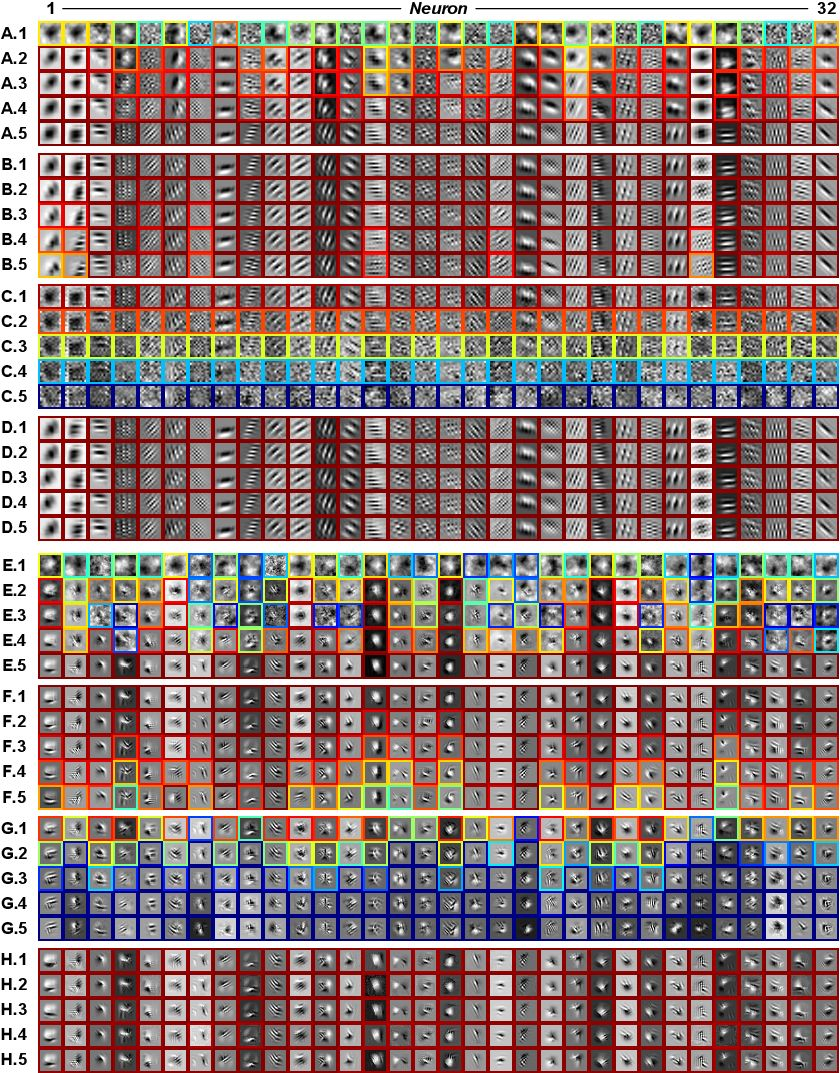
\includegraphics[width=0.9\textwidth]{Figs/pic1.pdf} \end{minipage}
\caption{
{\bf Visualization of shallow and deep representations.} (A) Optimal stimulus search trajectories of shallow neurons. Each column of (A) demonstrates the optimal stimulus search trajectory of one neuron, by showing the initial ${1}/{f}$ random stimulus in (A.1), resultant optimal stimulus in (A.5), and 3 intermediate stimuli corresponding to 3 largest second derivatives (i.e.~curvatures) of the fitness history in (A.2--4). (B) Invariance paths of shallow neurons. Each column of (B) demonstrates the invariance path search results of one neuron, starting from corresponding optimal stimulus as shown in (A.5) and moving away with distance constraints from $\delta = 0.1\pi$ to $0.5\pi$ as shown in (B.1--5) accordingly. (C) Selectivity paths of shallow neurons. Definitions follow (B). (D) Invariance subspaces of shallow neurons. Each column of (D) randomly shows 5 results out of 20 runs of invariance path searches at $\delta = 0.1\pi$. (E--H) Optimal stimulus search trajectories, invariance paths, selectivity paths, and invariance subspaces, of deep neurons, respectively. Definitions follow (A--D). Color indicates fitness (i.e.~response) of a neuron (definition of color map follows Fig.~\ref{fig:methods}).}
\label{fig:ind_res}
\end{FPfigure} %\end{figure}

Figure \ref{fig:ind_res}A and \ref{fig:ind_res}E exemplify the trajectories of optimal stimulus searches of 32 top-layer neurons from the best performing shallow network and 32 from the best performing deep network respectively. Worth to note, to further increase the searching speed, the initial stimulus is selected from 1000 ${1}/{f^{\alpha}}$ random stimuli with the best fitness, where $\alpha \in \left\lbrace -4,-3,-2,-1,0 \right\rbrace$, without sacrificing the nature of random initialization. From the results, two major differences can be observed. First, the fitness landscapes of deep neurons are significantly more complex than those of shallow neurons, as a large portion of searching trajectories for deep neurons actually go down then up before reaching the optima, which also suggests this numerical framework can handle non-convexity reasonably well. Second, the optimal stimuli of deep neurons are also relatively more complex (i.e.~consisting of more textural components) than those of shallow neurons (which are more uni-textured or Gabor-like).

%is also directly confirmed in this work. %to our knowledge, for the first time.

\begin{figure}
\centering 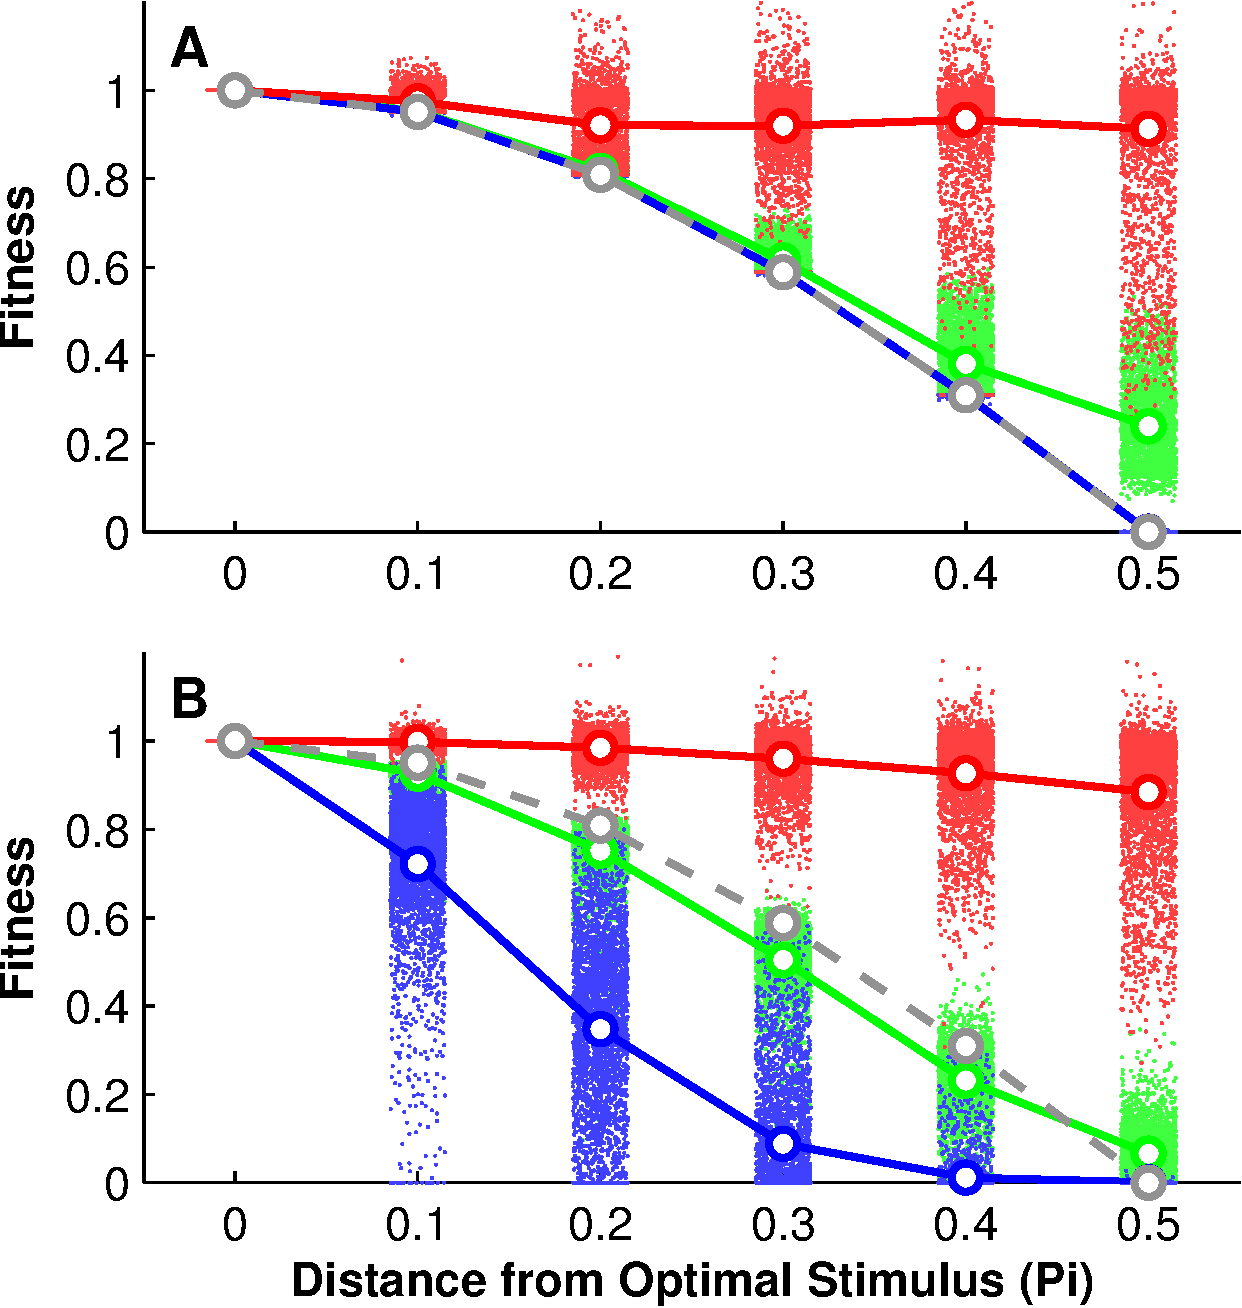
\includegraphics[width=0.5\textwidth]{Figs/e_fig3a_2-nup-crop.pdf}
\caption{
{\bf Comparison of shallow and deep fitness landscapes.} (A) Fitness-distance diagram of shallow neurons. Red, blue and green dots indicate results of invariance and selectivity path searches, and random walks. Means of results are plotted as solid lines in corresponding colors, and the cosine baseline curve as dashed line in gray. (B) Fitness-distance diagram of deep neurons. Definitions follow (A).}
\label{fig:ind_fdd} % NUMERICAL PRECISION!! WHY NO SLSC?
\end{figure}

Figure \ref{fig:ind_res}B/\ref{fig:ind_res}C and \ref{fig:ind_res}F/\ref{fig:ind_res}G exemplify the invariance/selectivity paths on the same sets of shallow and deep neurons as in Fig.~\ref{fig:ind_res}A and \ref{fig:ind_res}D. It can be observed that, while invariance paths are mostly phase changes and selectivity paths are leading toward meaningless noises (all at the same falloff rate) for shallow neurons, both types of paths consist of sophisticated shape deformations for deep neurons. Also, although most shallow neurons are selective to manually rotated optimal stimuli (i.e.~Gabor filters of different orientations) as well, their fitnesses still do not drop faster then the nonparametric numerical solutions as presented in Fig.~\ref{fig:ind_res}C. In fact, this intriguing difference generalizes across all shallow vs.~deep neurons tested in this work. As the fitness-distance diagrams shown in Fig.~\ref{fig:ind_fdd}, on average, though shallow neurons (Fig.~\ref{fig:ind_fdd}A) have good invariance (i.e.~red curve stays high), they do not have any selectivity (i.e.~blue curve drops slow and completely overlaps with baseline), while deep neurons (Fig.~\ref{fig:ind_fdd}B) show both good invariance and selectivity (i.e.~red curve stays high; blue curve drops fast). Random walks on the fitness landscape \cite{jones1995fitness}, shown as the green curve in Fig.~\ref{fig:ind_fdd}, can be defined as $f\left(\cos\left(\delta\right)\hat{x} + \sin\left(\delta\right)\tilde{x}\right)$ where $\tilde{x}$ is any random stimulus such that $\left\| \tilde{x} \right\| = 1$ and $\left\langle \hat{x},\tilde{x} \right\rangle = 0$, which can be obtained through random projection of $\mathrm{Null}\left(\hat{x}\right)$. Comparing the gaps between selectivity and random-walk curves in Fig.~\ref{fig:ind_fdd}A and \ref{fig:ind_fdd}B again shows the selectivity of deep neurons are in fact way more ``selective'' than of shallow neurons. To further characterize the invariance properties, multiple runs of invariance path searches are executed and results are visualized in Fig.~\ref{fig:ind_res}D and \ref{fig:ind_res}H. The diversity/dimensionality (i.e.~subspace capacity) of the ``invariance plateau'' (e.g.~the central high fitness region in Fig.~\ref{fig:methods}) of deep neurons is also more apparent than that of shallow neurons. Worth to note, it can be seen in Fig.~\ref{fig:ind_fdd} that small fractions of invariance path search results in fact have higher fitness than the optimal stimuli due to nature of non-convex problems, which however does not cause noticeable differences on resultant statistics.

\begin{figure}
\centering 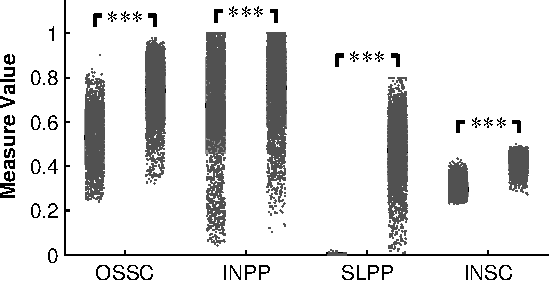
\includegraphics[width=0.5\textwidth]{Figs/e_fig23b-crop.pdf}
\caption{
{\bf Comparisons of shallow and deep representation measures.} Representation measures from left to right are, optimal stimulus spectral complexity (OSSC), invariance path potential (INPP), selectivity path potential (SLPP), and invariance subspace capacity (INSC), where data points from shallow networks (left distributions) and deep networks (right distributions) are shown side by side. Significances of differences of means are obtained through permutation tests, and $p < 0.001$ in all four measures. Sensitivity indexes ($d'$) between distributions of shallow and deep representation measures from left to right are 1.63, 0.42, 4.73, and 3.67.} %Means and standard deviations from left to right are, $0.53\pm0.12$, $0.74\pm0.13$, $0.67\pm0.22$, $0.76\pm0.17$, $0.00\pm0.00$, $0.47\pm0.14$, $0.30\pm0.03$, and $0.42\pm0.04$.
\label{fig:ind_mea}
\end{figure}

Comparisons of spectral complexities, invariance/selectivity path potentials, and invariance subspace capacities of shallow and deep neurons (i.e.~unit representations) are summarized in Fig.~\ref{fig:ind_mea}, where all measures are normalized to have analytical upper and lower bounds being 1 and 0. These measures break down the differences between shallow and deep representations, in addition to the straightforward representation separability/classifiability as used in previous studies \cite{donahue2014decaf, zeiler2014visualizing}. For instance, subtle differences of visual features have better chances being distinguished when the ``gap'' between invariance and selectivity curves (i.e.~the dynamic range of neuronal responses, or amplification ratio of differences) is large. The increasing of complexity in deeper neurons' preferred/optimal stimuli also agrees with neurobiological findings in higher visual cortical areas (e.g.~V2 and V4 \cite{hegde2000selectivity, pasupathy2001shape}). In addition, the highly structural representations of neurons from deep networks with purely random convolution kernels found in the experiments explain why such type of random deep networks can still have good performances, on top of the theoretical analysis of shallow networks \cite{saxe2011random}. 

%, which is also observed in this work (as shown in Fig.~\SFpef{})
%and futher point out the architecture is special/good
%[lecun's random]
%resize of OS

\subsection*{Good vs.~Bad Representations} %\label{sec:good_bad}

\begin{figure}
\centering 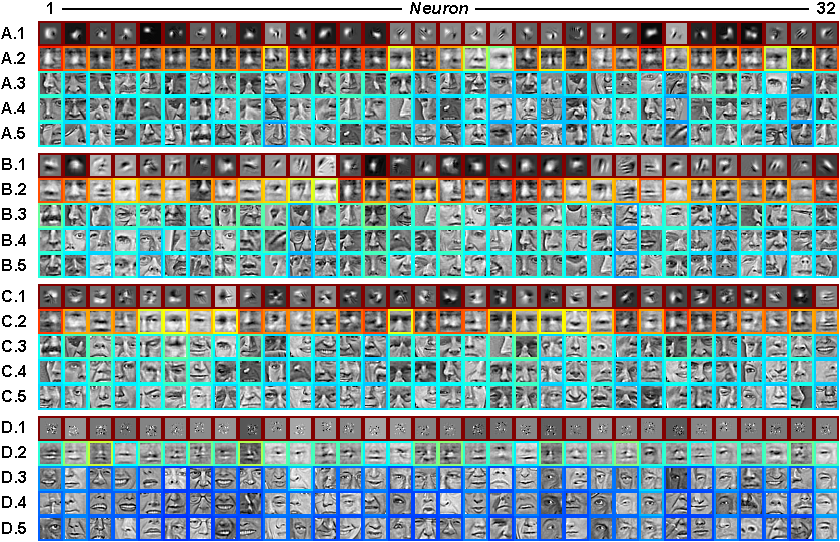
\includegraphics[width=0.9\textwidth]{Figs/pic2.pdf}
\caption{
{\bf Explanation power of optimal stimulus.} (A) Deep network with the best average explanation power of optimal stimulus. Each column of row (A.1) shows the optimal stimulus of the corresponding neuron. Each column of row (A.3--5) shows the task-related stimuli with the first, second, and third highest explainabilities (i.e.~inner-product distances to the optimal stimulus) respectively. Each column of row (A.2) shows the average of task-related stimuli with top 1\% explainabilities. (B--D) Deep networks with the second best, third best, and worst average explanation power of optimal stimulus, respectively. Definitions of rows follow (A). Color indicates explainability, and higher means better (definition of color map follows Fig.~\ref{fig:methods}).}
\label{fig:ind_exp}
\end{figure}

% how're stimuli sampled (face regions) from LFW-a
% DIFF BETWEEN FORMULA AND HERE??
%(calculated using only the top 1\% nearest task-related stimuli for visualization reasons; full set of task-related stimuli yields similar $R^2$ as well)
%Point out interesting cells. %reciprocal
% only deep nets, what runs are combined (by paragraph)
%; using all stimuli gives similar result of measure vs.~performance correlation.
%(though not improving $R^2$ when added into multiple correlation test ??)

To test how well optimal stimulus may linearly explain task-related stimuli and how the explanation power correlates with network's performance, 10,000 image patches are randomly sampled out of the predefined facial regions of pictures from the LFW-a dataset \cite{wolf2011effective} and compared against the optimal stimuli of all 32 top-layer neurons from all 100 deep networks. Figure \ref{fig:ind_exp} shows the results of best 3 (in \ref{fig:ind_exp}A--C) and worst 1 (in \ref{fig:ind_exp}D) networks in terms of explanation power. For simplicity and clarity of presentation, the explanation power measure is calculated using the top 1\% (i.e.~100) of the task-related stimuli with highest explainabilities, without biasing the results compared to using all task-related stimuli. It can be observed that, though none of the task-related stimuli (or arguably, of all natural stimuli) is highly similar to any optimal stimulus, there is an $R^2=0.36$ correlation (with details shown in Fig.~\SFexp{}) between network's explanation power and performance, and when alternatively comparing the average of the top 1\% of task-related stimuli and the optimal stimuli, the similarities become apparent. %representativeness

\begin{figure}
\centering 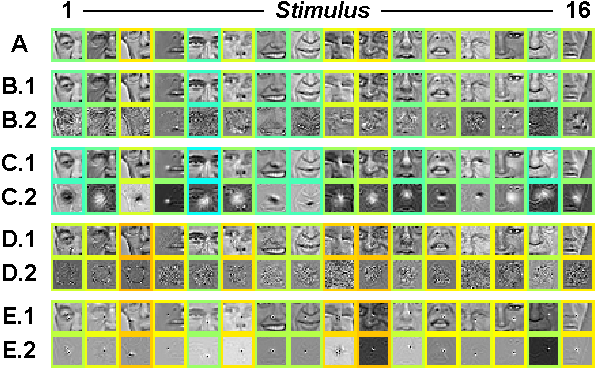
\includegraphics[width=0.5\textwidth]{Figs/pic3.pdf}
\caption{
{\bf Subspace alignment between invariance and selectivity paths and task-related stimuli.} (A) Reference stimuli used as starting points of invariance and selectivity path searches. (B) Best invariance subspace alignments. Each column of row (B.1) shows an invariance path search result with the best alignments against the principle component vector space of task-related stimuli (i.e.~the eigenface vector space). Each column of row (B.2) shows the difference between result in (B.1) and corresponding reference stimulus in (A) for better visual comparison. All columns do not necessary come from the same deep network. (C--E) Best selectivity subspace alignments, worst invariance subspace alignments, and worst selectivity subspace alignments, respectively. Definitions of rows follow (B). Color indicates alignment measure, and lower means better (definition of color map follows Fig.~\ref{fig:methods}).} % Show PCs or not? ref stimulus is not perfect either?
\label{fig:pop_aln}
\end{figure}

It has been shown that invariance and selectivity are extremely important for recognition in various modalities and species \cite{desimone1991face, ito1995size, quiroga2005invariant}; however, to how these properties directly affect the recognition performances remains unclear. To address this puzzle, starting from 16 randomly sampled reference stimuli (as shown in Fig.~\ref{fig:pop_aln}A), invariance and selectivity path searches are performed at $\delta = 0.1\pi$ using Eq.~(\ref{eq:I2}, \ref{eq:S2}) for population representations. Figure \ref{fig:pop_aln}B--E demonstrates the results of invariance and selectivity subspace alignment analyses. It can be observed that, good alignments (i.e.~sparser representations in principle component vector spaces) correspond to highly structural deformations or lighting changes, which are known to be important factors in visual recognition, while bad alignments correspond to mostly meaningless noises. The correlation between network's invariance/selectivity subspace alignment measure and performance is $R^2=0.19/0.31$ (with details shown in Fig.~\SFaln{}). Network's invariance subspace capacity (in terms of population representation), which though has an $R^2=0.15$ correlation as well, is in fact negatively correlated to network's performance (with details shown in Fig.~\SFinc{}), mainly due to the fact that poor performing network's invariance path search results are usually noisier (as depicted in Fig.~\ref{fig:pop_aln}D), and thus should be interpreted differently from unit representation cases. Invariance/selectivity path potentials for population representations, on the other hand, are weaker in explaining networks' performances (with $R^2=0.10/0.06$), due to the fact that all deep networks have high but less ordered invariance and selectivity (as the fitness-distance diagram shown in Fig.~\SFfda{}).

\begin{figure}
\centering 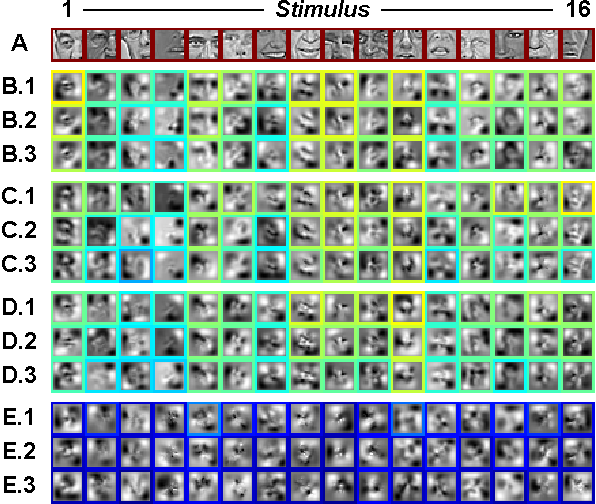
\includegraphics[width=0.5\textwidth]{Figs/pic4.pdf}
\caption{
{\bf Encoding specificity of task-related stimulus.} (A) Reference stimuli used as sources of representations. (B) Best encoding specificities. Each column of row (B.1--3) shows reconstructed stimuli of corresponding reference stimulus in (A) with top 3 SSIM measures (out of 10 reconstructions), from deep network of the best average encoding specificity. All columns do not necessary come from the same deep network. (C--E) Second best, third best, and worst encoding specificities, respectively. Definitions of rows follow (B). Color indicates SSIM measure, and higher means better (definition of color map follows Fig.~\ref{fig:methods}).}
\label{fig:pop_ens}
\end{figure}

%(see Text S\ref{?})
To further understand the meaning of population representation $r$ formed by a deep network $f$, the inverse function $f^{-1}\left( r \right)$ is approximated through the numerical optimization framework to reveal what kind of stimulus can drive the deep network to give output $r$. Instead of inverting randomly generated $r$, which may not have feasible or interpretable solutions, we use $r$ from known reference stimulus $x^{*}$, and study the encoding specificity and its relationship to performance. Figure \ref{fig:pop_ens} shows the reference stimuli (in \ref{fig:pop_ens}A), top 3 (in \ref{fig:pop_ens}B--D) and worst 1 (in \ref{fig:pop_ens}A) examples of encoding specificity, and the overall correlation between encoding specificity and performance is $R^2=0.41$ (with details shown in Fig.~\SFenc{}; SSIM measured using default settings of the standard implementation \cite{wang2004image} and different local window sizes yield similar correlations; other similarity measures like SNR, PSNR, and inner-product distance yield similar correlations as well). It can be observed that, though the reconstructed stimuli are overall of lower spatial frequencies, SSIM is still able to capture the relative similarity (e.g.~reconstructions of task-related stimulus 1 and 5).

\begin{figure}
\centering 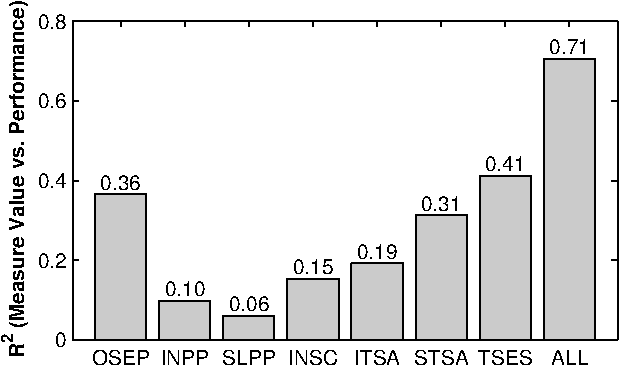
\includegraphics[width=0.5\textwidth]{Figs/e_fig7-crop.pdf}
\caption{
{\bf Spearman's correlations between deep network's representation measures and performance.} Representation measures from left to right are, optimal stimulus explanation power (OSEP), invariance path potential (INPP), selectivity path potential (SLPP), invariance subspace capacity (INSC), invariance vs.~task-related stimuli subspace alignment (ITSA), selectivity vs.~task-related stimuli subspace alignment (STSA), task-related stimulus encoding specificity (TSES), and all measures together (ALL) using linear multiple correlation analysis. Pearson's correlations following the same order are 0.37, 0.02, 0.02, 0.19, 0.17, 0.23, 0.39, and 0.69.}
\label{fig:all_R^2}
\end{figure}

%single best measure is...
%second best is ... and link to ...

Spearman's correlations between all representation measures and deep networks' performances are summarized in Fig.~\ref{fig:all_R^2}, and 71\% of the variance of deep networks' performances can be explained by the proposed measures altogether. These measures further break down the differences between deep representations and suggest features like network's explanation power, invariance and selectivity subspace properties, and encoding specificity against the task-related stimuli can be extremely important for the effectiveness of representations. Encoding specificity, as a single representation measure, can best explain the deep network's performance. Though bearing strong similarity to the invariance path search in terms of mathematical formulation, encoding specificity is in fact a radically different and complementary measure, since its numerical optimization is not constrained through distances to the reference stimulus, while distance constraints can induce \emph{a priori} similarities; it can better function as an unconstrained global characterization of the ``encoding landscape'' (i.e.~multivariate tuning landscape of a population) and estimate if the (reconstructed) stimuli that a deep network is invariant to are ``selective'' (i.e.~visually similar to original stimuli) at the same time. Explanation power of optimal stimulus is the second best single representation measure. Following the efficient coding theory \cite{barlow1961possible, laughlin1981simple}, one may exclude the possibility of an optimal stimulus looking highly similar to the task-related stimuli. Nevertheless, in a high-dimensional stimulus space, how to optimally construct the tuning landscape (and place the optimal stimuli) remains unclear, and whether the observed phenomenon (as shown in Fig.~\ref{fig:ind_exp}), in which optimal stimuli of well performing networks in fact are highly similar to the averages of neighboring task-related stimuli, is essential to the optimal tuning landscape still needs to be further studied. Worth to note, similar phenomenon was also reported in previous studies on well performing networks \cite{le2012building, simonyan2013deep}. Such ``linearities'' around the task-related stimuli out of highly nonlinear networks may also explain why natural stimuli can be more efficient in estimating the tuning of neurons \cite{talebi2012natural}. 

%1st-order predictive power vs 2nd-order (0.56, 0.58)
%For second-order representation measures provide relative lower 